\documentclass{extbook}
\usepackage[papersize={8.5in,11in},top=1in,bottom=1in]{geometry}
\RequirePackage{fix-cm}
\usepackage[T1]{fontenc}
\usepackage{lmodern}
\usepackage{fullpage}
\usepackage{titlesec}
\usepackage{parskip}
\usepackage{float}
\usepackage{url}
\usepackage{hyperref}
\usepackage{graphicx}
\usepackage{listings}
\usepackage{tcolorbox}
\usepackage{tabularx}
\usepackage{xcolor}
\usepackage{titlesec}
\usepackage{amsmath}
\renewcommand{\contentsname}{Contenido}
\renewcommand{\figurename}{Figura}
\renewcommand{\listfigurename}{Lista de figuras}
\renewcommand{\bibname}{Bibliografía}

\usepackage[fontsize=13.5pt]{fontsize}
\setlength{\parindent}{0pt}

\titleformat{\chapter}[display]
  {\bfseries\huge} % Estilo del título
  {\hfill\Large} % Alineación a la derecha
  {3ex} % Espaciado entre el número del capítulo y el título
  {\vspace{-5cm}\titlerule\vspace{1.5ex}\hfill} % Regla arriba y alineación del título a la derecha
  [\vspace{1ex}\titlerule] % Regla debajo del título


  \makeatletter
  \patchcmd{\chapter}
    {\if@openright\cleardoublepage\else\clearpage\fi}
    {\clearpage}
    {}{}
  \makeatother

  \definecolor{codegreen}{rgb}{0,0.6,0}
  \definecolor{codegray}{rgb}{0.5,0.5,0.5}
  \definecolor{codepurple}{rgb}{0.58,0,0.82}
  \definecolor{backcolour}{rgb}{0.95,0.95,0.92}
   
  \lstdefinestyle{mystyle}{
      backgroundcolor=\color{backcolour},   
      commentstyle=\color{codegreen},
      keywordstyle=\color{magenta},
      numberstyle=\tiny\color{codegray},
      stringstyle=\color{codepurple},
      basicstyle=\footnotesize,
      breakatwhitespace=false,         
      breaklines=true,                 
      captionpos=b,                    
      keepspaces=true,                 
      numbers=left,                    
      numbersep=5pt,                  
      showspaces=false,                
      showstringspaces=false,
      showtabs=false,                  
      tabsize=2
  }
   
  \lstset{style=mystyle}


\begin{document}
\begin{titlepage}
    \begin{center}
        {\huge \textbf{Universidad Tecnológica de Panamá}}\\
        \vspace{3mm}
        {\Large \textbf{Centro Regional De Veraguas}}

        \begin{figure}[H]
            \centering
            
\includegraphics[scale = 0.07]{Imagenes/utp.png}
            
\includegraphics[scale = 0.58]{Imagenes/fisc.png}
        \end{figure}
        {\Large \textbf{Facultad de Ingeniería de Sistemas Computacionales}}\\
        \vspace{5mm}
        
        {\Large \textbf{Curso: Circuitos Lógicos}}\medskip
        
        {\Large \textbf{Profesor: Abel Rodriguez}}

        \rule{\linewidth}{0.75mm}\\

            {\Large \textsc{Informe de laboratorio 5}} 
        \rule{\linewidth}{0.75mm}\medskip

        {\Large \textbf{Estudiantes}}\\
        \vspace{5mm}
        {\Large \textbf{Elbin Puga, Arland Barrera, Priscila Ortega y Steven Espinosa}}
        \vfill
        {\Huge \textbf{2024}}

    \end{center}
\end{titlepage}
\tableofcontents
\listoffigures
\chapter{Marco Teórico}
\section{Las Compuertas Lógicas}

Una compuerta lógica es un dispositivo electrónica que en función de los valores de entrada otorga un resultado o una salida determinada, son la base de la electrónica digital. Se utilizan no solo en electrónica si no que conceptualmente sus fundamentos se aplican en otras áreas de la ciencia, Mecánica hidráulica o neumática por ejemplo. vamos a comentar el funcionamiento de algunas compuertas lógicas básicas y sus tablas de verdad.

\subsection{Compuerta AND (BUFFER)}

Para que una compuerta AND entregue un uno a la salida, todas las entradas deben tambien estar en uno, basta con que alguna con lo este para que en la salida se vea un cero, “Si condición uno Y condición dos Y condición tres se cumplen, entonces la salida sera verdadera.” En términos simbólicos a la operación se la conoce con el símbolo “.” o “ˆ“.
\begin{figure}[H]
    \centering
    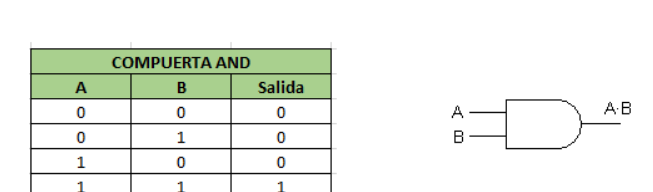
\includegraphics[scale = 0.70]{Imagenes/AND.png}
    \caption{Compuerta AND}{Fuente: Internet}
\end{figure}


\subsection{COMPUERTA NOT}
Todo lo que ingresa por la entrada, a la salida entrega lo opuesto, si ingresa un estado alto “1” a la salida se vera un estado bajo “0” por ejemplo, tiene una sola entrada.

\begin{figure}[H]
    \centering
    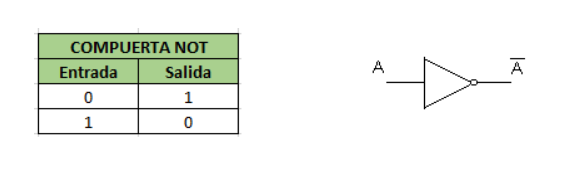
\includegraphics[scale = 0.70]{Imagenes/NOT.png}
    \caption{Compuerta NOT}{Fuente: Internet}
\end{figure}

\subsection{COMPUERTA OR}
Esta compuerta es diferente a la AND, basta con que una de las entradas este en estado alto para que automáticamente la salida pase a estar en estado alto, “Si condición uno O condición dos O condición tres entonces la salida sera verdadera”. En términos simbólicos a la operación se la conoce con el símbolo +.

\begin{figure}[H]
    \centering
    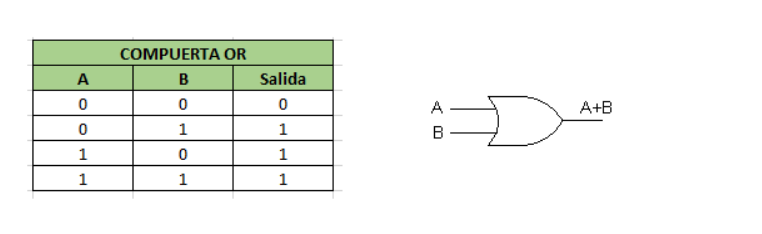
\includegraphics[scale = 0.7]{Imagenes/OR.png}
    \caption{Compuerta OR}{Fuente: Internet}
\end{figure}

\subsection{COMPUERTA XOR de 2 entradas}

Este tipo de compuertas son una derivación de las compuertas básicas que comentamos al comienzo, tienen una condición de salida no tan transparente como los casos anteriores, pero son muy utilizadas en el mundo de la electrónica digital.
Para un sistema de dos entradas la ecuación característica es la siguiente.

Para un sistema de dos entradas la ecuación característica es la siguiente.

\begin{equation}
    F = A \bigoplus B
    F = \neg A B +  A \neg B
\end{equation}

Como se puede ver, la salida deja de ser tan intuitiva con en los casos anteriores, de manera que es necesario diagramar la tabla de verdad para calcular correctamente el resultado.
Como dato memotecnico, para una compuerta XOR de dos entradas podemos decir que a la salida va un uno si las dos entradas son distintas.

\begin{figure}[H]
    \centering
    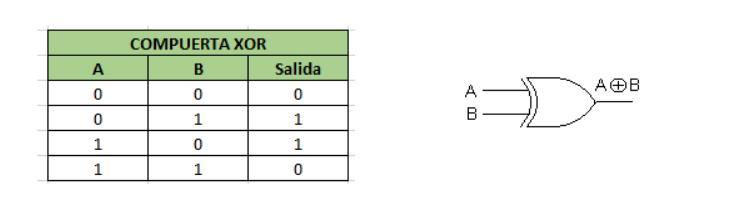
\includegraphics[scale = 0.70]{Imagenes/XOR.png}
    \caption{Compuerta XOR}{Fuente: Internet}
\end{figure}

\subsection{COMPUERTA XOR (de tres entradas)}
Funciona de la misma manera que la de dos entradas, solo que es mas largo el calculo, puesto que primero tenemos que hacer el calculo con dos entradas y luego sumarle la tercera, esta operatoria aplica para una compuerta XOR de cualquier cantidad de entradas, solo es necesario estar atento en el calculo y listo.

Como dato memotecnico, para una compuerta XOR de tres entradas podemos decir que la salida sera un uno si la cantidad de unos en la entrada es impar.

\begin{figure}[H]
    \centering
    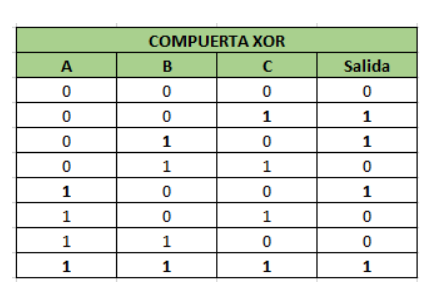
\includegraphics[scale = 0.7]{Imagenes/XOR3.png}
    \caption{Compuerta XOR (3 entradas)}{Fuente: Internet}
\end{figure}



\chapter{Introducción}
\input{2 Introduccion/introduccion.tex}
\chapter{Cuerpo de trabajo}
\section{Tema: Introducción a la placa Arduino}
\section{Objetivos generales}
\input{3 Cuerpo de trabajo/3.2_ob_generales.tex}
\section{Objetivos Específicos}
\begin{itemize}
    \item Comprobar las tablas de verdad de puertas lógicas y sus combinaciones.
    \item Conocer las principales Puertas Lógicas, su simbología y comportamiento.
    \item Utilizar Arduino para comprobar el comportamiento de los mismos.
\end{itemize}
\section{Materiales}
\input{3 Cuerpo de trabajo/3.4_materiales.tex}
\chapter{Desarrollo}
\section{Circuitos propuestos}
\section{Circuitos desarrollados}
\input{4 Desarrollo/circuitos_fotos.tex}
\chapter{Conclusiones}
Los operadores lógicos son piedras angulares en el mundo de la programación. Estos actúan como los cimientos que sostienen la complejidad de los algoritmos y permiten que las máquinas «piensen» y tomen decisiones basadas en instrucciones precisas. A través de este artículo, hemos explorado cómo estas herramientas, aparentemente simples, combinan y se entrelazan para crear sistemas más sofisticados y adaptativos.

Al trabajar con Arduino, y en programación en general, comprender estos operadores es fundamental. A medida que los dispositivos se vuelven más inteligentes y las expectativas sobre su rendimiento crecen, la lógica detrás de sus decisiones se vuelve cada vez más crucial. Ya sea para encender una luz bajo ciertas condiciones, activar una alarma o controlar un sistema complejo, estas estructuras de control son esenciales.

El poder de la programación radica en su capacidad para traducir la lógica humana en instrucciones que una máquina pueda comprender y ejecutar. Y, en este proceso, los operadores lógicos son el lenguaje universal que facilita esta traducción.

A medida que continuamos avanzando en la era digital, donde la interacción entre humanos y máquinas se vuelve cada vez más íntima y compleja, es esencial que tengamos una sólida comprensión de estas herramientas. La programación, en su esencia, es el arte de la lógica y la resolución de problemas, y los operadores lógicos son las herramientas con las que esculpimos soluciones en este arte.

Agradezco a todos los lectores por acompañarnos en este viaje a través de los operadores lógicos en Arduino. Sea cual sea su nivel de experiencia, espero que este artículo haya proporcionado claridad, inspiración y una mayor apreciación por la belleza subyacente de la lógica en programación.
\addcontentsline{toc}{chapter}{Bibliografía}

\begin{thebibliography}{99}
    \bibitem{i_AND}
    \textit{A. P. Mendoza. “Puertas y Funciones Lógicas”. Circuitos Digitales 2018-II C5 B.} Disponible en\url{https://circuitosdigitalesc5b2018.blogspot.com/2018/08/2-marco-teorico-2.html}
\end{thebibliography}
\chapter{Anexos}
\section{Data de los materiales usados}
\input{8 Anexos/anexo.tex}
\section{Alcance de la aplicación de este laboratorio a futuro}
\end{document}
